\documentclass[12pt]{article}

\usepackage{amssymb,amsmath,amsthm}
\usepackage{graphicx} % Package for including figures
%\usepackage{psfrag,color}
\graphicspath{ {.}}

\theoremstyle{definition}
\newtheorem{thm}{Theorem}[section]
\newtheorem{lem}[thm]{Lema}
\newtheorem{prop}[thm]{Proposition}
\newtheorem*{cor}{Corrolary}

\theoremstyle{definition}
\newtheorem{defn}{Definition}[section]
\newtheorem{conj}{Conjecture}[section]
\newtheorem{exmp}{Example}[section]


\title{Report: Homework 3 Math/CS 471}
\author{Teo Brandt and Brennan Collins}
\date{\today}   % Activate to display a given date or no date


\begin{document}
\maketitle

\begin{abstract}
This report will explore two methods of approximating the following integral
\[
I=\int_{-1}^{1}e^{cos(kx)}dx,
\]
for \(k=pi\text{ or }pi^{2}\). The first method is known as the trapezoidal rule and the second as Gauss quadrature.
\end{abstract}

\section{Trapezoidal Rule}
The trapezoidal rule is given by the following expression
\[
\int_{X_{L}}^{X_R}f(x)dx\approx h\bigg(\frac{f(x_{0})+f(x_{n})}{2}+\sum_{i=1}^{n-1}f(x_{i})\bigg)
\]
where the grid is given by \(x_{i}=X_{L}+ih\text{, }i=0,...,n\text{, }h=\frac{X_{R}-X_{L}}{n}\).
\section{Gauss Quadrature}
From the definition offered in \cite{HW} Gauss quadrature involves the location of the grid-points and weights, \(\omega_{i}\), are chosen so that the order of the approximation to the weighted integral
\[
\int_{-1}^{1}f(z)w(z)dz\approx \sum_{i=0}^{n}\omega_{i}f(z_{i}),
\]
is maximized. (The function \(w(z)\) is positive and integrable. In this report we will only consider the case when \(w(z)=1\) in order to simplify things.

\section{Results}
\begin{figure}[h]
\caption{Error plot for trapezoidal and Gauss estimations}
\centering
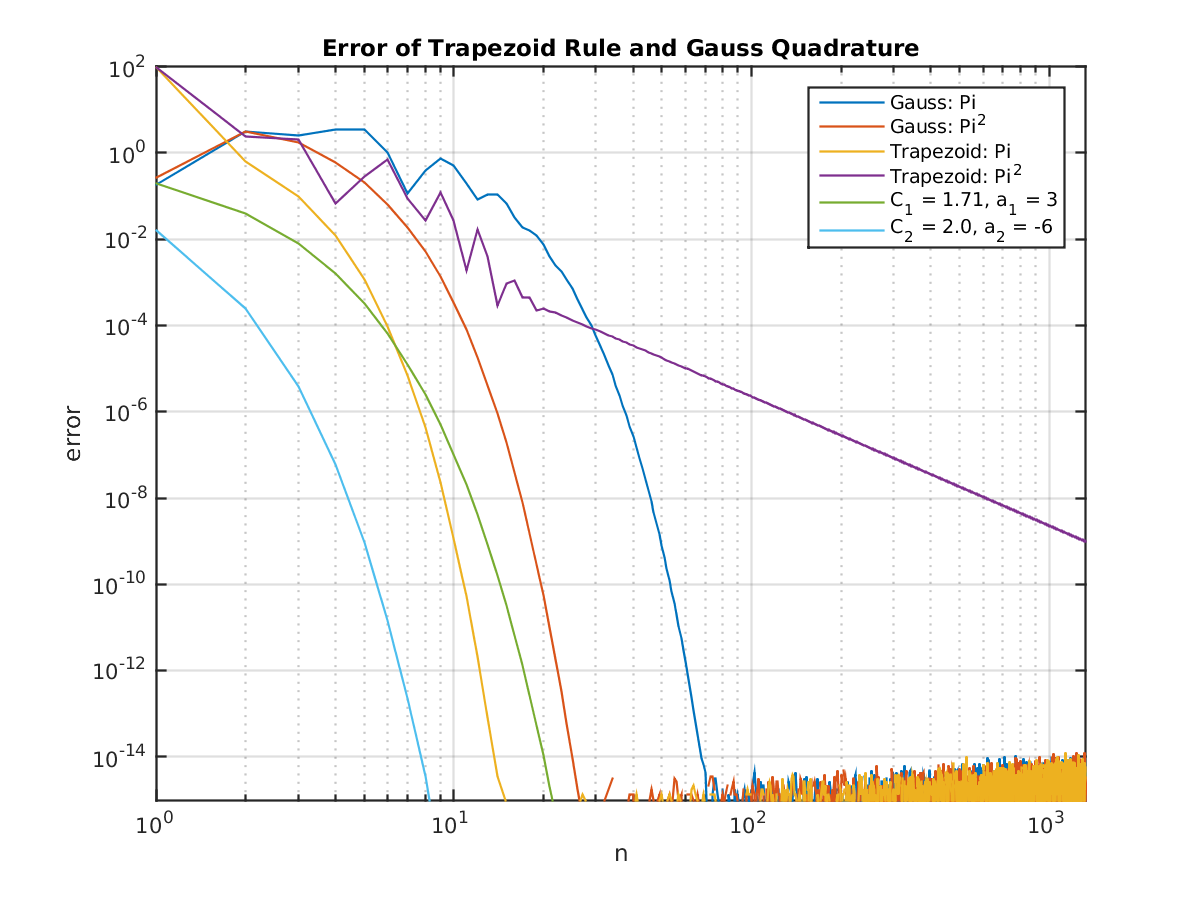
\includegraphics[width=1\textwidth]{ErrorPlot}
\end{figure}

In the figure shown above, different rates of convergence are observed for each of the methods and for each of the values of \(k\). The trapezoidal method where \(k=\pi^{2}\) is the only case in which the order of the method may be read from the slope of its plot. This slope is \(\approx -3\) which is consistent with the theory as shown in \cite{Wiki}
\[
error=-\frac{(b-a)^{2}}{12N^{2}}\big[f\prime(b)-f\prime(a)\big]+\textit{O}(N^{-3})
\]
The error plot above (Fig.1) shows that the fastest rate of convergence occurred with the trapezoid approximation when \(k=\pi\), followed by the Gauss quadrature approximations (\(k=\pi^{2}\) converging faster than \(k=\pi\)), and then the slowest rate of convergence was demonstrated by the trapezoid approximation with \(k=\pi^{2}\). This observation is interesting because the trapezoid approximation with \(k=\pi\) converges faster than expected.
\\ 
For Gauss quadrature the error was expected to decrease as \(e(n)\approx C^{-an}\). We tried \(C_{1} = 1.71\) and \(C_{2} = 2\) with respective \(a_{1} = 3\) and \(a_{2} = -6\). The second plot appeared to resemble the Gauss approximation.

\newpage
\section{Appendix}
To run the program, simply navigate to Homework3/Code and enter the command \textit{"perl approx\_error.p"}. This may take a minute to complete, but when it concludes a png file named \textit{"ErrorPlot.png"} will be created with the plots of the errors for both the Trapezoidal Rule and Gauss Quadrature for both values of k (\(\pi\) and \(\pi^{2}\)) and the file is saved in the Report directory.

\newpage
\begin{thebibliography}{9}
\bibitem{HW} 
Daniel Appelo
\textit{Homework 3}. 
referenced Sep. 26, 2015

\bibitem{Wiki}
Trapezoidal rule. \today. Retrieved from\\
\textit{https://en.wikipedia.org/wiki/Trapezoidal\_rule\#Error\_analysis}
\end{thebibliography}
\end{document} 
